\section{Implementation}\label{impl}
This section presents an overview of the implementation of SCache -- a distributed in-memory shuffle data storage system with a DAG co-scheduler. Here we use Spark as an example of DAG framework to illustrate the workflow of shuffle optimization. We will first present the system overview in Subsection \ref{arch} while the following two subsections focus on the two constraints on memory management.

\subsection{System Overview}\label{arch}
SCache consists of three components: a distributed in-memory shuffle data storage system, a DAG co-scheduler and a daemon inside Spark. As shown in Figure \ref{fig:arch}, for the in-memory storage system, SCache employs the legacy master-slaves architecture like GFS \cite{gfs}. The master node of SCache coordinates the shuffle blocks globally with application context. The worker node reserves memory to store blocks
The coordination provides two guarantees: (a)data is stored in memory before tasks start and (b)data is scheduled on-off memory with all-or-nothing and context-aware constraints to benefit all jobs. 
The daemon bridges the communication between Spark and SCache. The co-scheduler is dedicated to pre-schedule reduce tasks with DAG information and enforce the scheduling results to Spark scheduler.

When a Spark job starts, the DAG will be first generated. Spark DAG scheduler recursively visits the dependencies from the last RDD. While traversing RDDs reversely, the DAG computing pipeline will be cut off if a RDD has one or more shuffle dependencies. These shuffle dependencies among RDDs will then be submitted through a RPC call to SCache master by a daemon process in Spark driver. For each shuffle dependency, the shuffle ID (an integer generated by Spark), the type of partitioner, the number of map tasks, and the number of reduce tasks are included. The SCache master will store the information of one RPC call as a shuffle scheduling unit. If there is a specialized partitioner, such as range partitioner, in the shuffle dependencies, the daemon will insert a sampling program before the dependent RDDs. We will elaborate the sampling procedure in the Section \ref{sampling}.

For the hash partitioner, when a map task finishes computing, the SCache daemon process will transfer the shuffle map output from Spark executor to the reserved memory through memory copy.
At the same time, the map task will end and the slot will be released after the memory copy without blocking disk write.
When the shuffle map output is received, the SCache worker will then notify the master of the block information with the reduce size distribution in this block (see map output in Figure \ref{fig:shuffle}).
If the collected map output data reach the observation threshold, the SCache co-scheduler will then run the scheduling Algorithm \ref{hminheap} and \ref{mhminheap} to pre-schedule the reduce tasks and then broadcast the scheduling result.
The pre-fetching of shuffle data starts as soon as each worker receives the scheduling results.
More specifically, when a map task is finished, each node will receive a broadcast message. SCache worker will filter the reduce tasks ID that will be launched on itself and starts to pre-fetch shuffle data from the remote. After the blocks of shuffle map output are transferred, the SCache worker will flush these blocks to disk to free memory space.
Before the reduce stage starts, Spark DAG Scheduler first generates a task set for this stage with different locality levels --- \textit{PROCESS\_LOCAL, NODE\_LOCAL, NO\_PREF, RACK\_LOCAL, ANY}.
To enforce SCache pre-scheduled tasks -- node mapping, we insert some lines of codes in Spark DAG Scheduler.
For RDDs with shuffle dependencies, Spark DAG scheduler will consult SCache master to get the preferred node for each partition and set \textit{NODE\_LOCAL} locality level on corresponding reduce tasks.

When the scheduled reduce tasks start, the shuffle input data can be fetched from reserved memory in SCache worker through daemon process. As soon as the data is consumed by the reduce task, it will be flushed to the disk.

\subsubsection{Reservoir Sampling}\label{sampling}
If the submitted shuffle dependencies contain a range partitioner or a customized non-hash partitioner, the SCache master will send a sampling request to the daemon in Spark driver. The daemon then inserts a sampling job before the corresponding RDD. The sampling job uses a reservoir sampling algorithm \cite{reservoir} on each partition of RDD. For the sample number, we set the size to $3 \times number\ of\ partitions$ for balancing overhead and accuracy (it can be tuned by configuration). The sampling job randomly selects some items and performs a local shuffle with partitioner (see Figure \ref{fig:sample}). At the same time, the items number is counted as the weight. These sampling data will be aggregated by reduce ID on SCache master to predict the reduce partition size. After the prediction, SCache master will call Algorithm \ref{mhminheap} and \ref{hminheap} to do the scheduling.

\begin{figure}
	\centering
	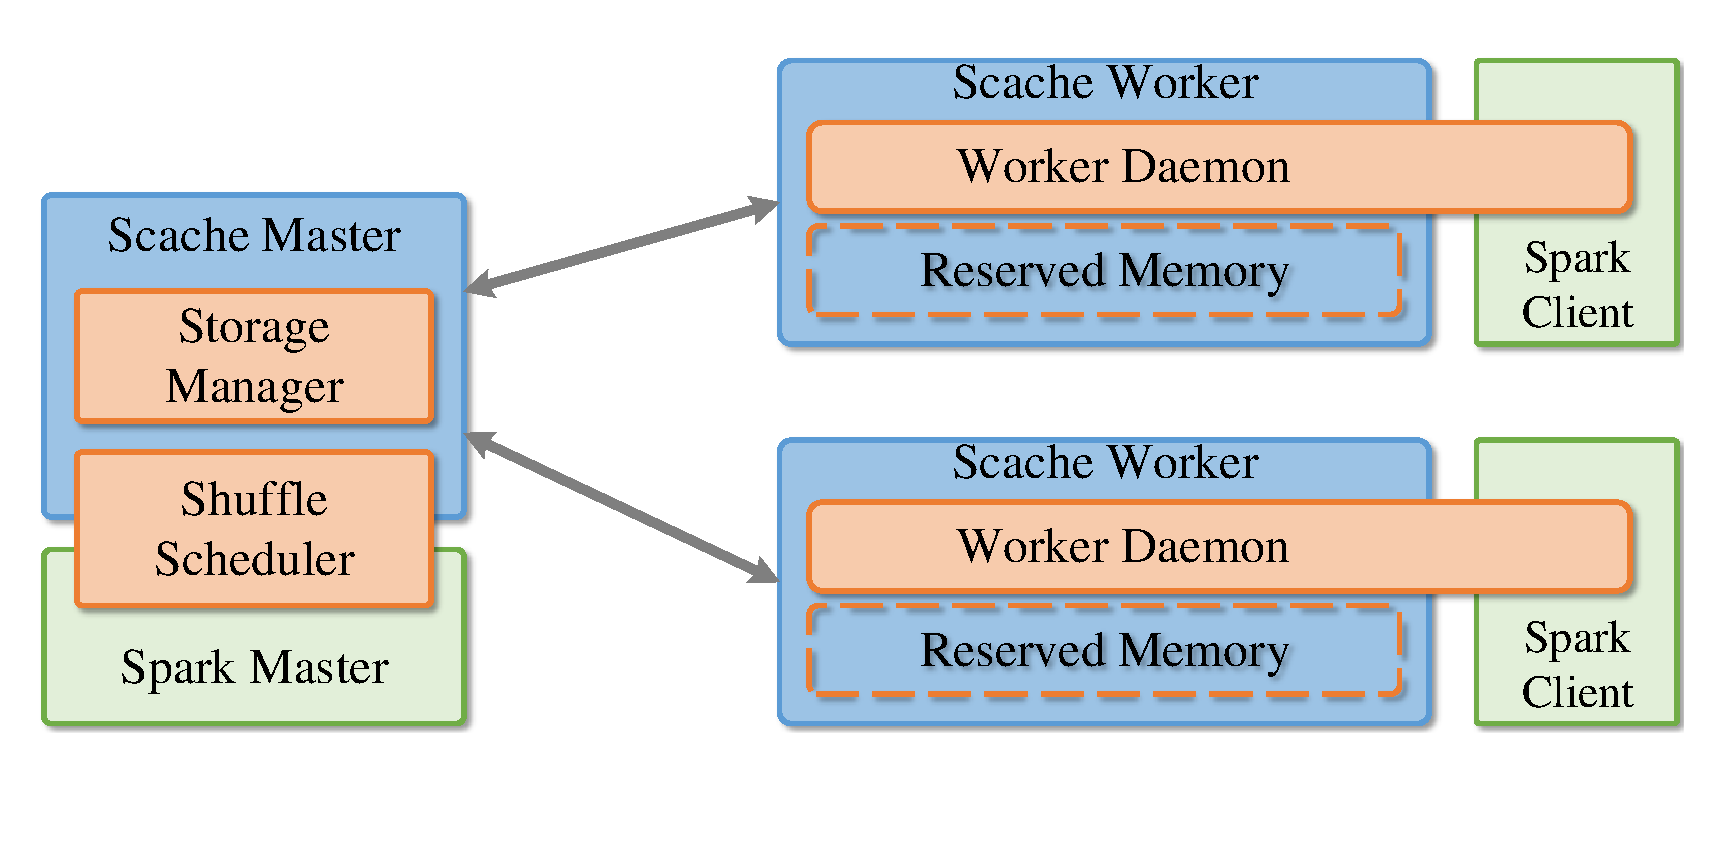
\includegraphics[width=0.9\linewidth]{fig/arch}
	\caption{SCache Architecture}
	\label{fig:arch}
\end{figure}
\begin{figure}
	\centering
	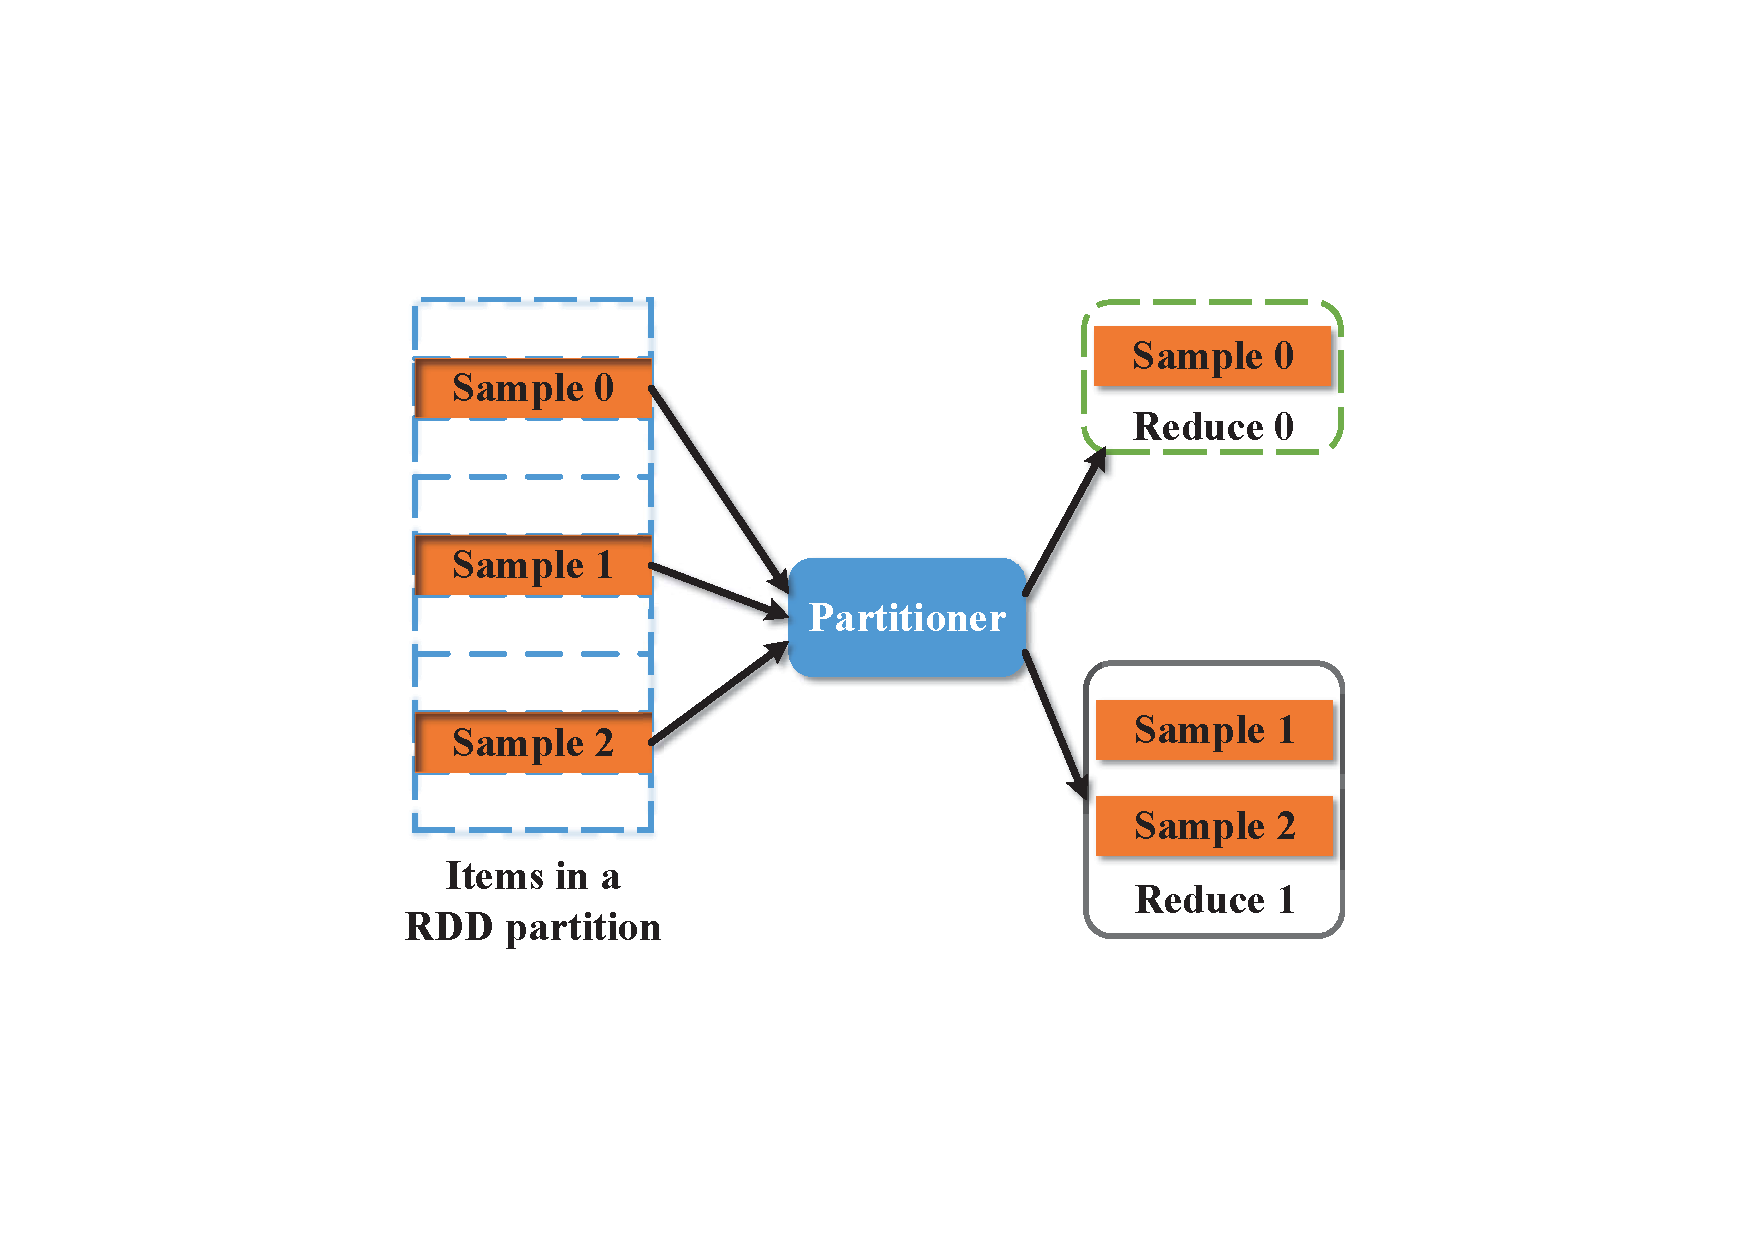
\includegraphics[width=0.6\linewidth]{fig/sample}
	\caption{Reservoir Sampling of One Partition}
	\label{fig:sample}
\end{figure}

\subsection{Memory Management}\label{memorymanage}
As mentioned in section \ref{observation}, though the shuffle size is relatively small, memory management should still be cautious enough to limit the effect of performance of DAG framework.
When the size of cached blocks reaches the limitation of reserved memory, SCache flushes some of them to the disk temporarily, and re-fetches them when some cached shuffle blocks is consumed or pre-fetched. To achieve maximum overall improvement, SCache leverages two constraints to manage the in-memory data --- all-or-nothing and context-aware-priority.

\subsubsection{All-or-Nothing Constraint}
Memory cached shuffle blocks can speed up the reduce task execution process. But this acceleration of a single task is necessary but insufficient for a shorter stage completion time. Based on the observation in section \ref{multi}, in most cases one single stage contains multi-rounds of tasks. If one task misses a memory cache and exceeds the original bottleneck of this round, that task might become the new bottleneck and further slow down the whole stage. PACMan \cite{pacman} has also proved that for multi-round stage/job, the completion time improves in steps when $n\times number\ of\ tasks\ in\ one\ round$ of tasks have data cached simultaneously. Therefore, the cache of shuffle blocks need to match the demand of all tasks in one running round at least. We refer to this as the all-or-nothing constraint.

According to all-or-nothing constraint, SCache master leverages the pre-scheduled results to determine the bound of each round, and set corresponding blocks as minimum unit of storage management.
For those incomplete units, SCache will mark them as the lowest priority.
% Following the all-or-noting constraint can maximum the improvement in stage completion time by using reserved memory efficiently.

\subsubsection{Context-Aware-Priority Constraint}
When the size of cached shuffle data exceeds the reserved memory, SCache should pick up victims and flush them to disk.
SCache master first searches for the incomplete units and flush all belonging blocks to disk cluster-widely.

But what if all the units are completed in the cluster? Traditional cache replacement schemes, such as MIN \cite{min}, only maximize cache hit ratio without considering the application context in DAG computing. But the cached shuffle blocks are only read exactly once (without failure), the hit ratio is actually meaningless in this scenario.
In addition, directly applying them might violate the all-or-nothing constraint.
To decide the priorities among units, SCache makes decision in two dimensions -- \textit{inter-shuffle units} and \textit{intra-shuffle unit}.
\begin{itemize}[noitemsep]
	\item Inter-shuffle units: SCache master follows the scheduling scheme of Spark to determine the inter-shuffle priority. For a FAIR scheduler, Spark balances the resource among task sets, which leads to a higher priority for those with more remaining tasks. The more remaining tasks a stage have, the more storage units left unconsumed. So SCache sets priorities from high to low in a descending order of remaining storage units of a shuffle unit. For a FIFO scheduler, Spark schedules the task set that is submitted first. So SCache sets the priorities according to the submit time of each shuffle unit.
	\item Intra-shuffle unit: SCache also needs to decide the priority among storage units inside a shuffle unit. According to the task scheduling inside a task set of Spark, the tasks with smaller ID will be scheduled firstly under one locality level. Based on this, SCache can assign the storage unit with larger task ID with lower priority.
\end{itemize}
In a word, SCache selects the shuffle unit with the lowest inter-shuffle priority and evicts the storage units according to intra-shuffle priority.



% \subsubsection{Fault Tolerance}
% To prevent the machine failure in cluster leading to inconsistency SCache, the master node will log the meta data of shuffle register and scheduling on the disk. Since we remove the shuffle transfer from the critical path of DAG computing, the disk log will not introduce extra overhead to the DAG framworks. Note that the master can be implemented with Apache ZooKeeper \cite{zookeeper} to provide constantly service to DAG framework.
% At the same time, every work node will send a heartbeat to master to report status. If a failure of work node is detected, the master will the do a simple re-schedule. For those scheduled shuffle units, the master assgins the tasks to other workers with more lightweight workload evenly. Then the new assigned worker will fetch the data again. For the incomplete in memory map blocks on the failure node, SCache simply ignore them since DAG framework will schedule the failure map tasks on another node.
